\documentclass[smaller]{beamer}
\usepackage{beamerarticle}
\mode<presentation> {
  \usetheme[width=80pt]{Berkeley}
  \useinnertheme{circles}
  \usecolortheme{sidebartab}
  \setbeamercolor{structure}{fg=blue}
  % or ...

%  \setbeamercovered{transparent}
  % or whatever (possibly just delete it)
}

%\usepackage[russian]{babel}
%\usepackage[cp1251]{inputenc}
\usepackage[utf8]{inputenc}
\usepackage[english,russian]{babel}
%\usepackage[pdftex,unicode]{hyperref}
%\usepackage{amsfonts}

%\usepackage{color}
%\usepackage{amsmath}
%\usepackage{amssymb}
%\usepackage{graphics}
%\usepackage{epsfig}
%\usepackage{color}
%\usepackage{times}
%\usepackage{array}
%\usepackage{../lectures}
\usepackage{listings}
\usepackage[pdftex,unicode]{hyperref}
%\usepackage[noend]{algorithmic}
\usepackage[noend]{algorithm}
\usepackage[noend]{algpseudocode}

%\usepackage{algorithm2e}

\newcommand{\eA}{ {\bf A} }
\newcommand{\eB}{ {\bf B} }


%\newcommand{\mod}{\mbox{mod}}
%\usepackage[T1]{fontenc}
%\usefonttheme{professionalfonts}
\usefonttheme{serif}
% Or whatever. Note that the encoding and the font should match. If T1
% does not look nice, try deleting the line with the fontenc.


\title{Fuzzy patterns sdcfsd } % (optional, use only with long paper titles)

\author[Вишневский] % (optional, use only with lots of authors)
{В.\,В.\,Вишневский\inst{1}}
\institute[МГУ ВМК, ММП] % (optional, but mostly needed)
{
  \inst{1}
  МГУ, ВМиК, каф. ММП
}

\date[Patterns] % (optional, should be abbreviation of conference name)
{}
% - Either use conference name or its abbreviation.
% - Not really informative to the audience, more for people (including
%   yourself) who are reading the slides online

\AtBeginSubsection[] {
  \begin{frame}<beamer>
    \frametitle{План}
    \tableofcontents[currentsection,currentsubsection]
  \end{frame}
}
\begin{document}

\begin{frame}
  \titlepage
\end{frame}

\begin{frame}
  \frametitle{План}
  \tableofcontents
  % You might wish to add the option [pausesections]
\end{frame}

\section{Введение}
\subsection{Где встречается задача}

\begin{frame}
  \frametitle{Поиск закономерностей}
\begin{itemize}
  \item Поведение -- важна иерархия, точные временные интервалы,
  \item белковые структуры(биологические последовательности) -- огромные объемы данных, биологическая информация о структуре,
  \item распространение сигналов по сетям(компьютерным и биологическим) -- большие объемы данных, можно использовать кластеризацию,
  \item анализ потребительской корзины -- не важна последовательность, $min\_support$.
  \end{itemize}
\end{frame}

\section{Т-Паттерны}

\begin{frame}
  \frametitle{Данные}
  \begin{itemize}
  \item Элементраные события (event types): $A,B,C,D$,
  \item у каждого события есть времена появления: $t_{A_1},...,t_{A_N}$ 
  \end{itemize}
  
    \begin{center}
      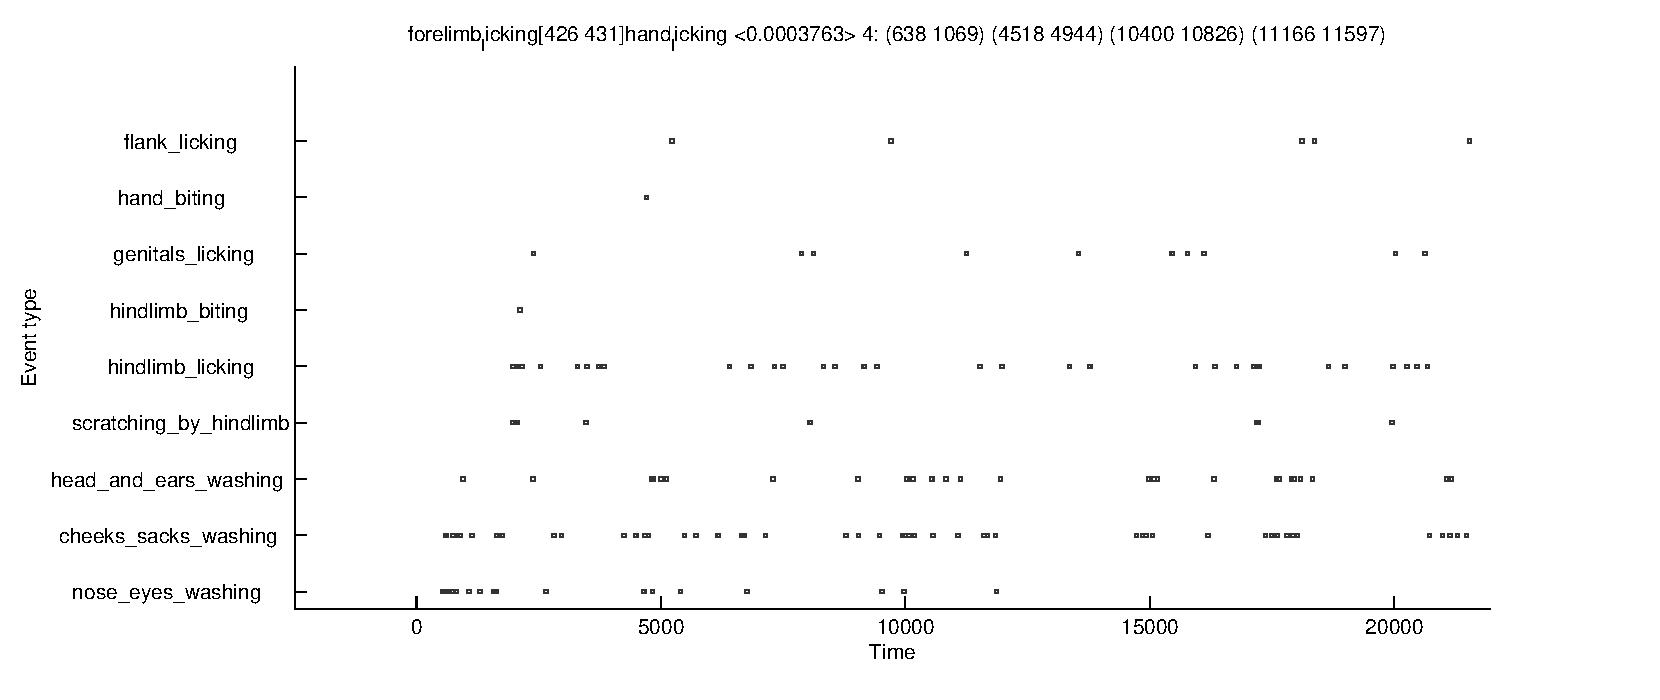
\includegraphics[scale=0.35]{TS.eps}
    \end{center}
\end{frame}


\begin{frame}
  \frametitle{Критический интервал}
 
      События связываются в паттерны критическими интервалами.

      Критический интервал -- это связь между двумя паттернами, означающая, что второй паттерн встречается в некотором промежутке после первого чаще, чем ожидется.
	
  \begin{center}
      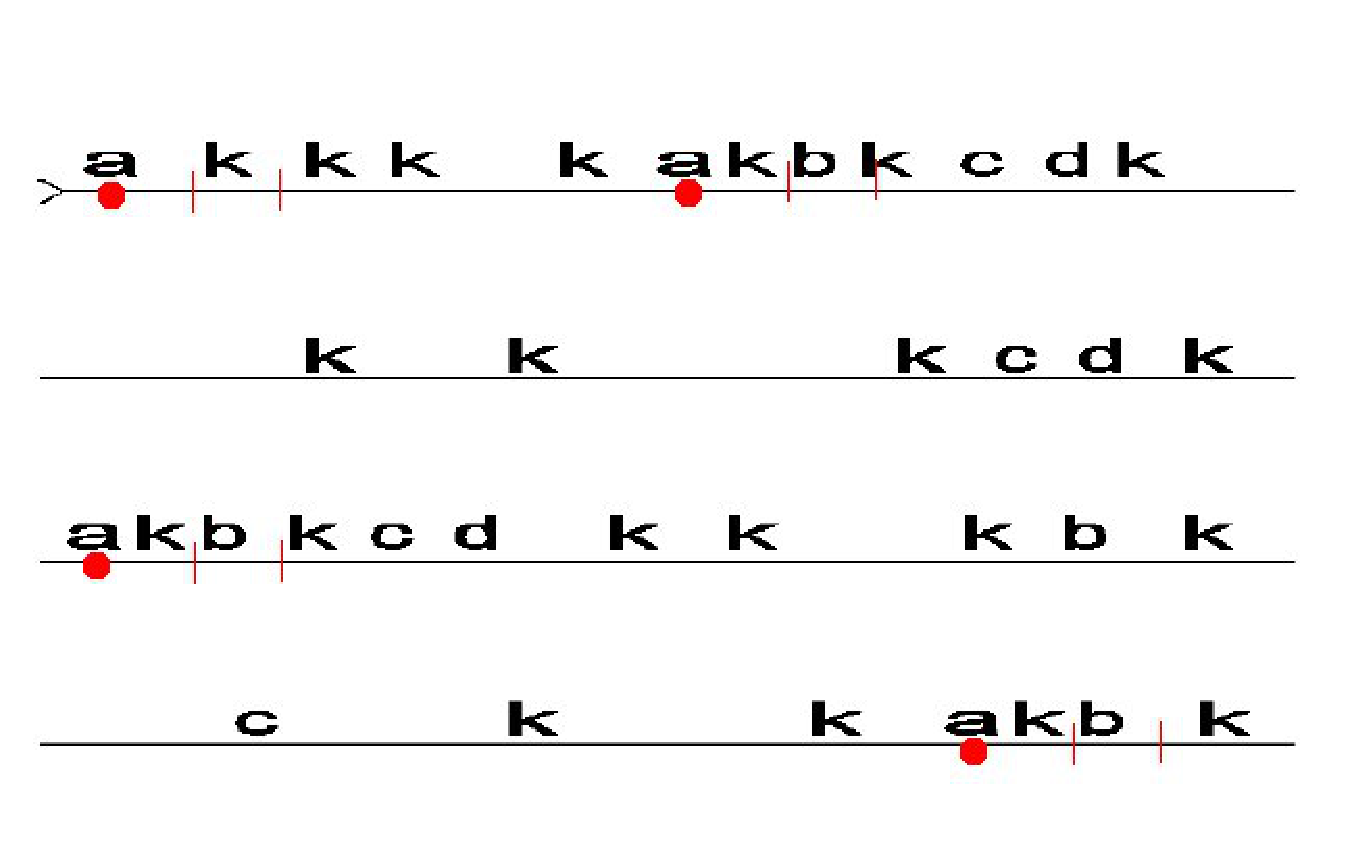
\includegraphics[scale=0.22]{TSCI.eps}
    \end{center}
$$\rho = P(\geqslant N_{\eA\eB}) = 1 - \sum_{i=0}^{N_{\eA\eB}-1}C_{N_{\eA}}^i( 1-P(\neg\eB)^d )^iP(\neg\eB)^{N_{\eA}-i}.$$
\end{frame}

\begin{frame}
  \frametitle{Процедура поиска}
  Пока добавляются новые паттерны:
  \begin{itemize}
  \item Для всевозможных пар паттернов, пытаемся найти связывающий их критический интервал,
  \item удаление неполных копий и паттернов-дубликатов.
   \end{itemize}

\end{frame}

\begin{frame}
  \frametitle{Параметры метода}
  Какие условия можно задавать на паттерны:
  \begin{itemize}
  \item Уровень значимости,
  \item условия на элементарные события, входящие в паттерн,
  \item длина критической связи,
  \item стратегия поиска критических связей,
  \item пересечение паттернов.
   \end{itemize}
\end{frame}

\section{Нечеткие паттерны}
\begin{frame}
  \frametitle{Предпосылки}
  \begin{itemize}
  \item Еще раз: Т-Паттерны очень чувствительны к пропускам в данных,
  \item новый тип паттернов, 
  \item схожий с Т-Паттернами метод поиска,
  \item правдоподобие паттерна в каждой точке.
   \end{itemize}
\end{frame}

\begin{frame}
\frametitle{Представление паттерна}
 \begin{itemize}
  \item Паттерн состоит из элементарных событий,
  \item каждое событие паттерна характеризуется смещением и разбросом от предыдущего события(гармошка),
  \item либо от предыдущего мат. ожидания(занавеска),
  \item $P=A[\mu_A,\sigma_A]B[\mu_B,\sigma_B]C[\mu_C,\sigma_C]$
 \end{itemize}
\begin{left}
\begin{tabular}[t]{p{12em}|p{12em}}
    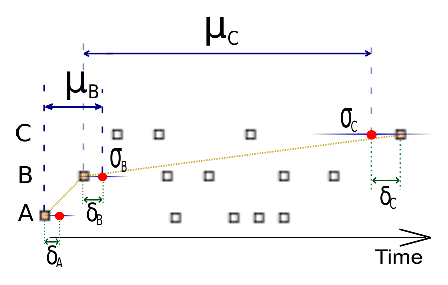
\includegraphics[scale=0.6]{il1.eps} & 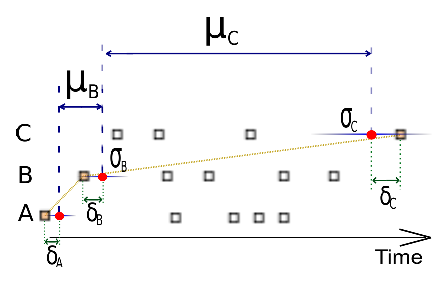
\includegraphics[scale=0.6]{il2.eps}\\

\end{tabular}
\end{left}
\end{frame}  

\subsection{Правдоподобие паттерна}
\begin{frame}
  \frametitle{Функция потерь}
  \begin{itemize}
  \item Штраф за пропуск $x$ событий из паттерна длины $N$:
  $$
  f_{LOSS}(x,N)= \begin{cases}
   \exp\bigl(-\frac{\lambda x}{N}\bigr), & x < N, \\
   0,                                    & x=N.
   \end{cases}
  $$
  \item $\lambda$ определяет уровень нечеткости паттернов.
   \end{itemize}
   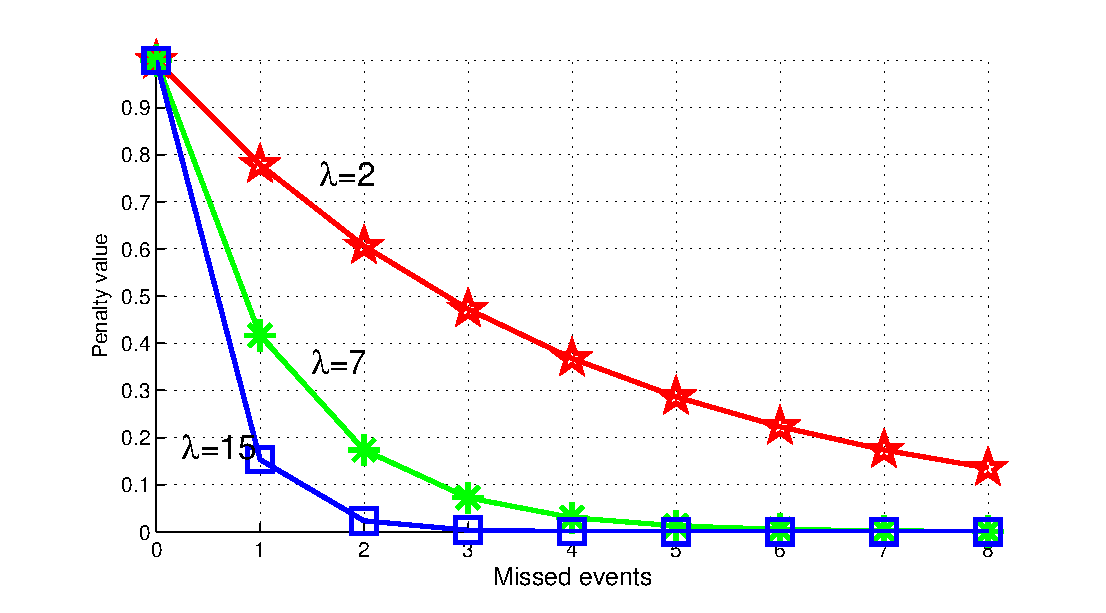
\includegraphics[scale=0.35]{MB_LF.eps}
\end{frame}

\begin{frame}
  \frametitle{Правдоподобие}
   $$L_P(\varepsilon)=f_{LOSS}(N_-,N)\prod_{i=1}^{N}\biggl( \frac1{\sqrt{2\pi}\sigma_i }\biggr)  \prod_{i=1}^{N_+}\exp\biggl(- \frac{\delta_i^2}{2\sigma_i^2}\biggr) $$
   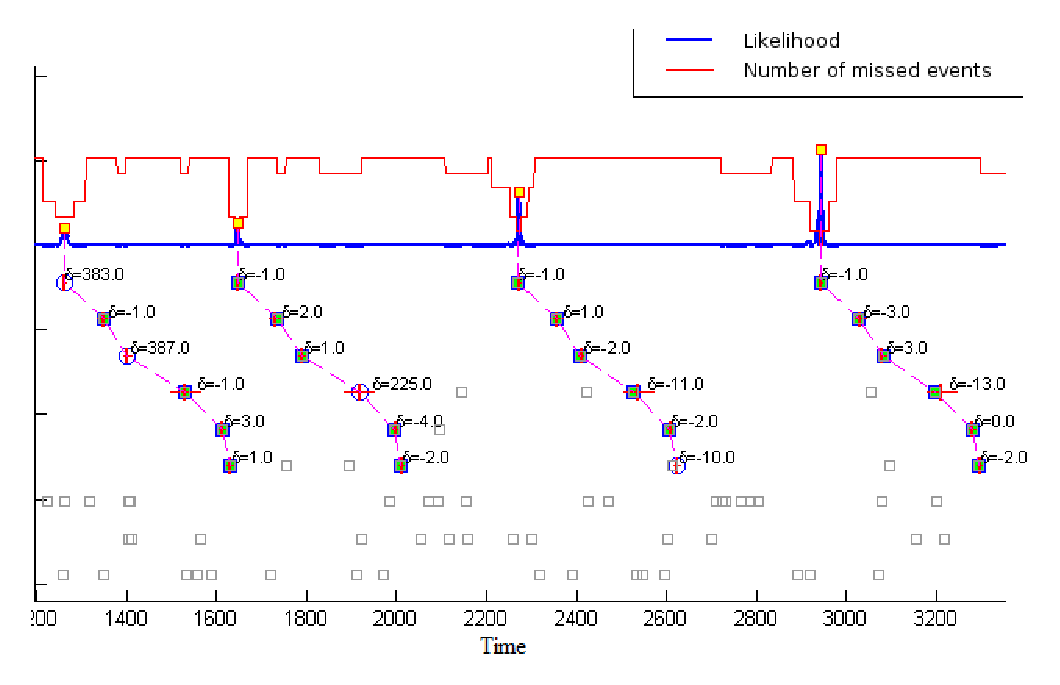
\includegraphics[scale=0.4]{norm_12_of_14.eps}
\end{frame}

\begin{frame}
  \frametitle{Правдоподобие}
   Правдоподобие можно считать с конца, или начиная с $i$-го события.
    $$L_{P,m}=L_P(\varepsilon+\sum_{j=1}^m\mu_j)$$
   \begin{center}
   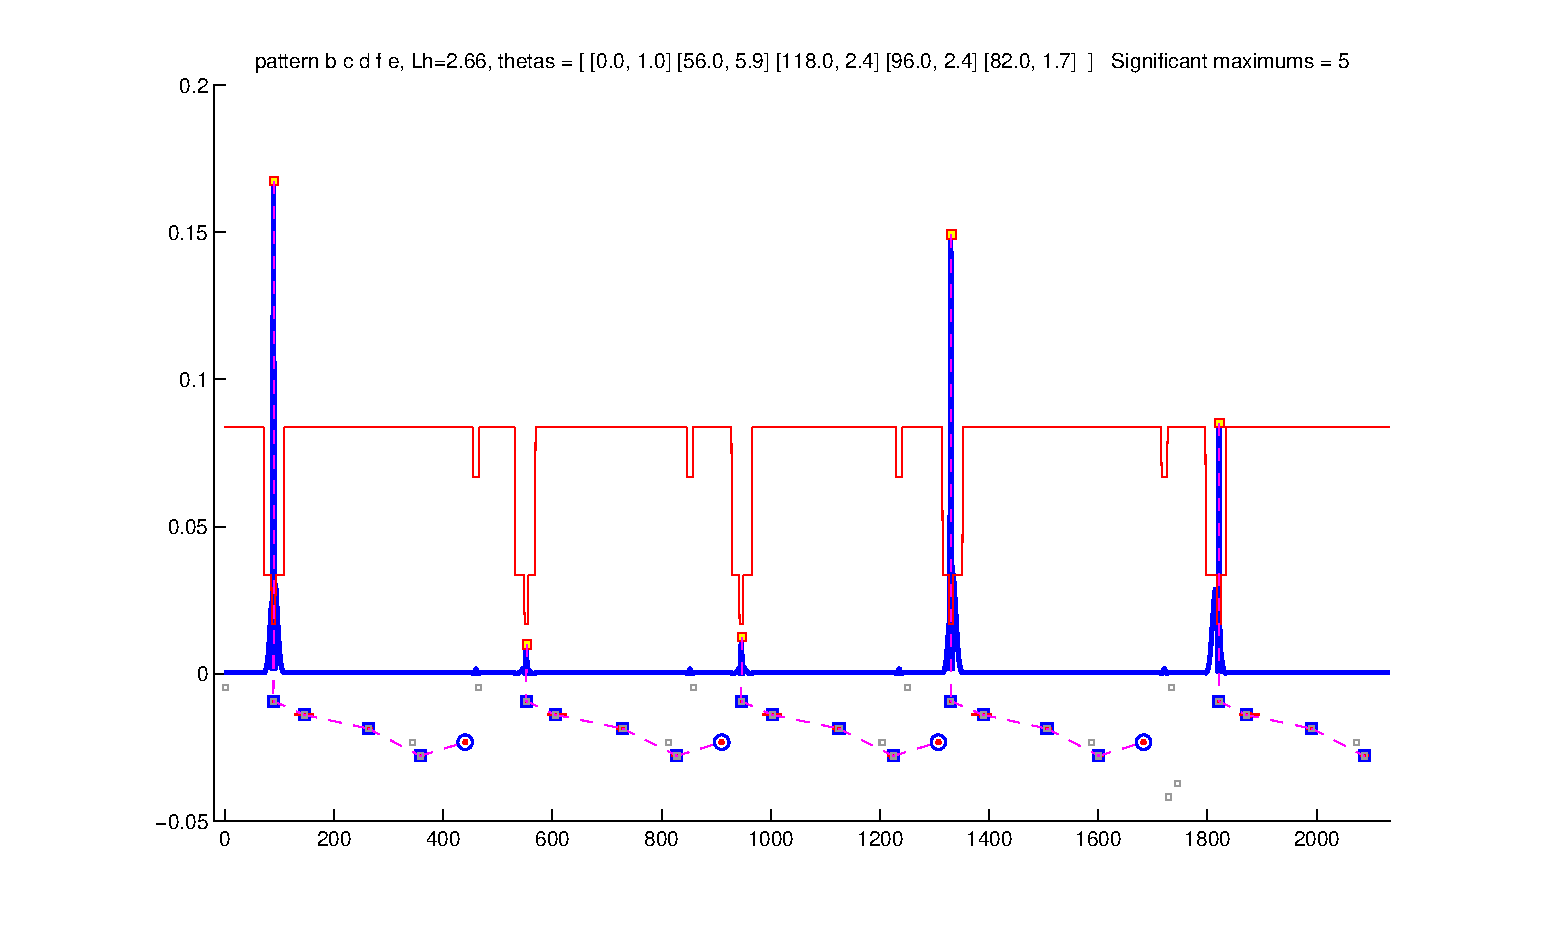
\includegraphics[scale=0.2]{pat1.eps}
   \\
   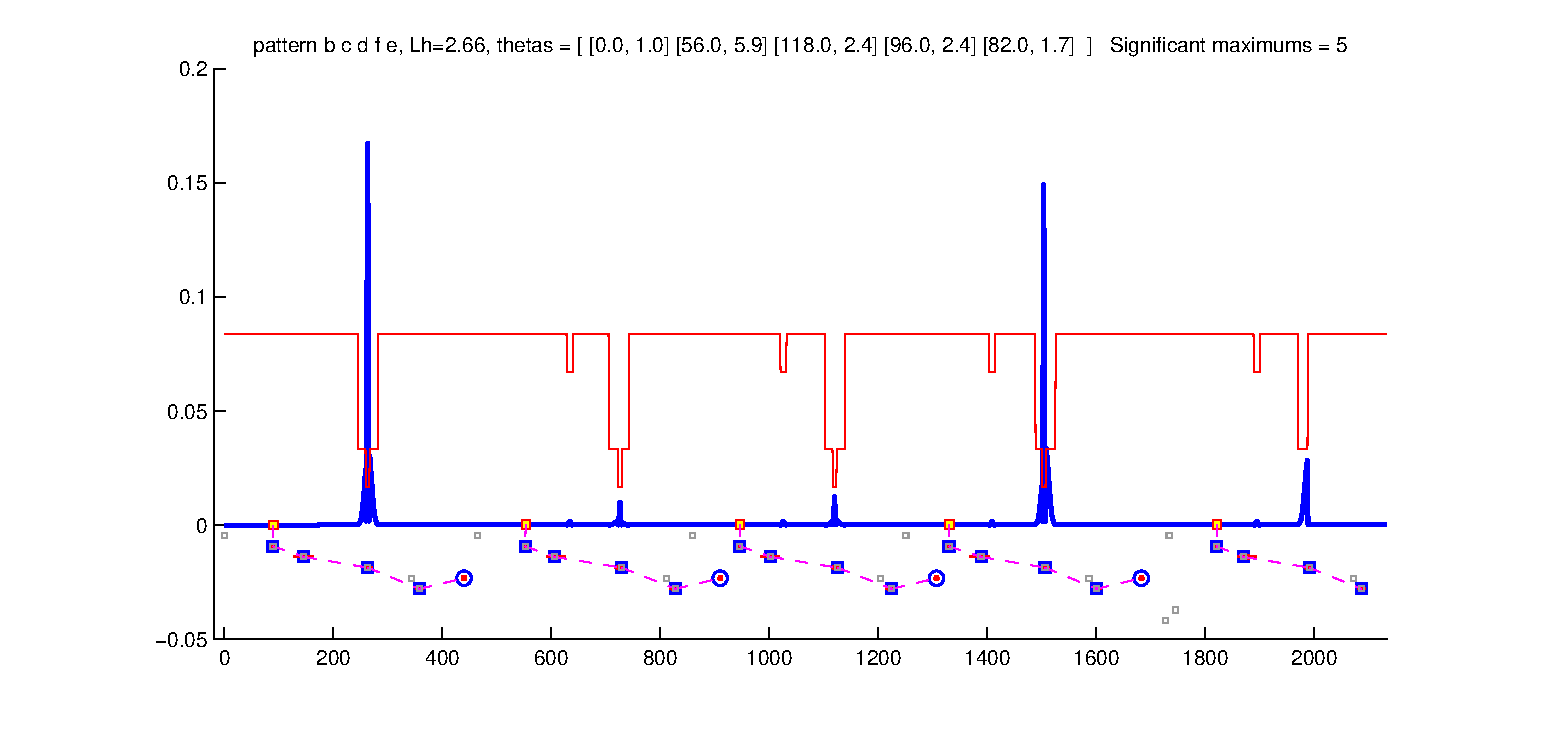
\includegraphics[scale=0.2]{pat2.eps}
   \end{center}
\end{frame}

\subsection{Статистический критерий}
\begin{frame}
  \frametitle{Межточечное распределение}
  \begin{itemize}
   \item Рассматриваем распределение расстояний между концом левого и началом правого паттерна,
   \item отсечение окном ширины $M$,
   \item вводим $g_{\mu,\sigma}(\rho_l)=\exp\bigl(-\frac{(\rho_l-\mu)^2}{2\sigma^2}\bigr)$~-- это статистическая модель связи между событиями,
   \item подсчитываем $k=\sum_{l=1}^Q w_lg_{\mu,\sigma}(\rho_l).$
   \end{itemize}
   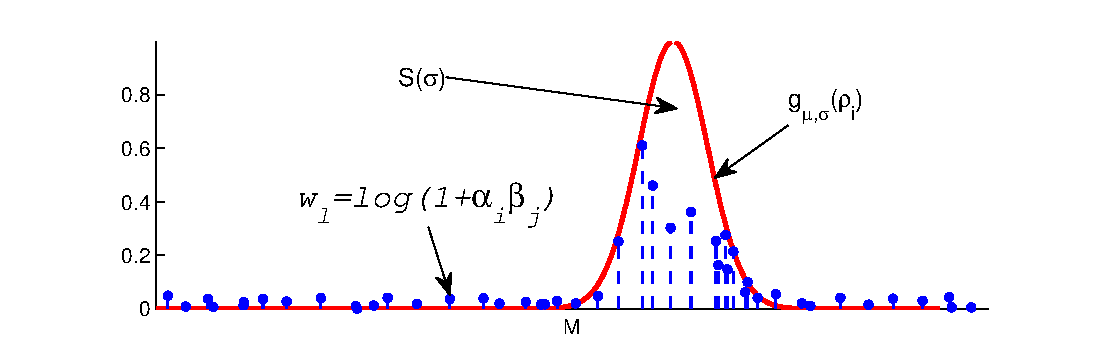
\includegraphics[scale=0.4]{weights.eps}
\end{frame}

\begin{frame}
  \frametitle{Гипотеза о случайности распределения}
  \begin{itemize}
    \item Если в данных нету закономерностей:
    \begin{itemize}
        \item  с.в. $w$ и $\rho_l$~-- независимы,
        \item  $\rho_l \in U[0,M]$,
        \item $Y=\sum_{l=1}^Qw_lg_{\mu,\sigma}(\rho_l)$, 
    \end{itemize}
    \item Используя Ц.П.Т, можно показать, что:
    $$Y\sim \mathcal{N}\biggl( \frac{\sum_{i=1}^Q w_i}MS, \frac1{M^2}\biggl[ MS\sqrt{2}\sum_{i=1}^Q w_i^2-\frac{(\sum_{i=1}^Q w_i)^2}QS^2 \biggr] \biggr)$$
    \item ищем $\mu$ и $\sigma$:
    $$\frac{k-\mathbb{E}Y}{\sqrt{\mathbb{D}Y}}\to\min_{\mu,\sigma},$$
    \item сравниваем с квантилью нормальмального распределения; $\omega$.
   \end{itemize}
\end{frame}

\subsection{Удаление паттернов}
\begin{frame}
  \frametitle{Виды <<лишних>> паттернов}
  \begin{itemize}
   \item {\bf Дубли:} (AB)(CD), (ABC)D,
   \item {\bf Неполные копии:} например, (BCD) не встречается вне (ABCD).
   \item похожесть паттернов по вектору правдоподобия $\overrightarrow{L}$, коэффициент корреляции:
   $$cor(\overrightarrow{L_1}, \overrightarrow{L_2}) = \frac{\overrightarrow{L_1}\overrightarrow{L_2}^T}{\sqrt{\overrightarrow{L_1}\overrightarrow{L_1}^T}\sqrt{\overrightarrow{L_2}\overrightarrow{L_2}^T}}$$
   \end{itemize}
\end{frame}

\begin{frame}
  \frametitle{Процедура удаления}
  
  Есть паттерн $P_1$ и $P_2$.
  Если все события, которые входят в $P_1$ так же 
  входят в $P_2$ и  $\exists m: cor(\overrightarrow{L_{P_1,m}}, \overrightarrow{L_{P_2,1}}) > \nu$, то  
  $P_1$ удаляется.
   
   
\end{frame}


\subsection{Результаты экспериментов}
\begin{frame}
  \frametitle{Модельные данные}
  
        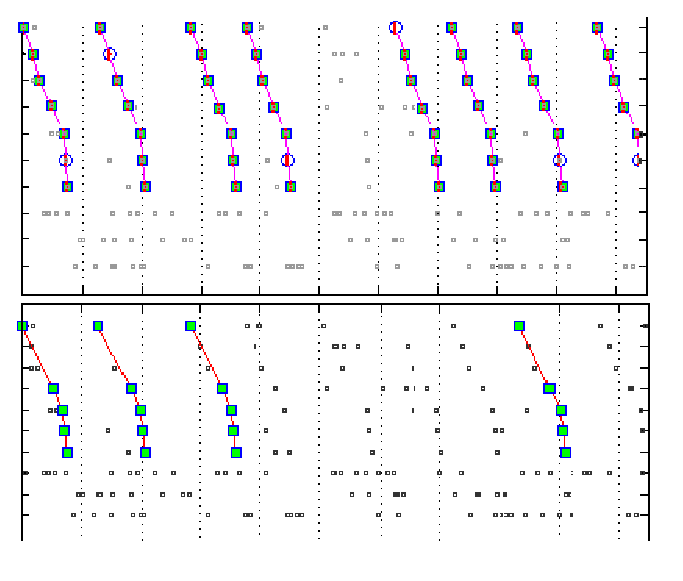
\includegraphics[scale=0.6]{comp.eps}

\end{frame}


\begin{frame}
  \frametitle{Реальные данные}
          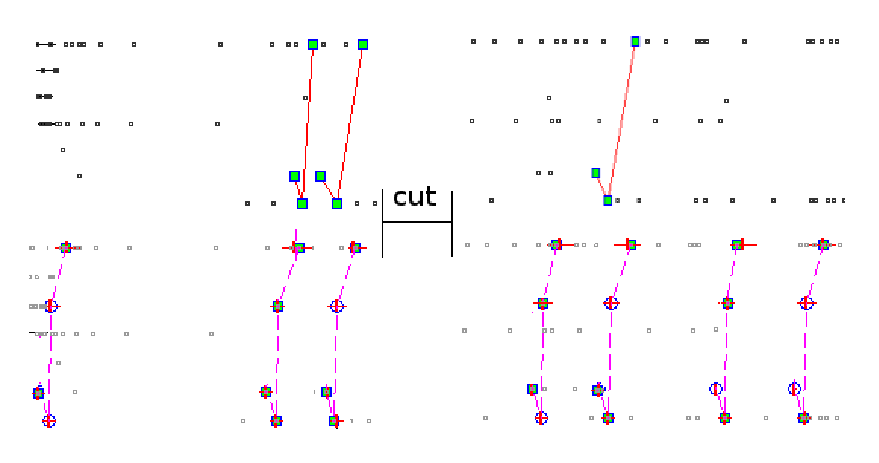
\includegraphics[scale=0.6]{exa.eps}
 \end{frame}

\begin{frame}
  \frametitle{Эксперименты}
   \begin{itemize}
   \item Хорошо работает процедура удаления неполных паттернов и дубликатов,
   \item иногда плохо срабатывает поиск смещений и дисперсий,
   \item долго работает,
   \item нечеткие паттерны все же ищутся.
   \end{itemize}
 \end{frame}


\section{Другие алгоритмы}
\subsection{P-Patterns}

\begin{frame}
  \frametitle{P-patterns}
Sheng Ma and Joseph L. Hellerstein. <<Mining Partially Periodic Event Patterns With Unknown Periods>>. IBM T.J. Watson Research Center Hawthorne, NY 10532. [50902.pdf]
  \begin{itemize}
    \item Решается задача поиска паттернов в коммуникационных сетях,
    \item заданым окном ширины $ w $ ведется поиск ассоциативных правил,
    \item поиск периодов с помощью FFT и критерия $\chi^2$,
    \item параметры: 
\begin{tabular}[t]{|p{3em}|p{11em}|p{6em}|}
\hline
\delta & time tolerance, & predefined\\
\hline
$w$    & time window & predefined\\
\hline
$minsup$ & minimum support for p-pattern & predefined\\
\hline
$p$ & period length & to be found\\
\hline   
$\bf{A_1}$ & subset of event types. & to be found\\
\hline   
\end{tabular}
  \end{itemize}
\end{frame}

\begin{frame}
  \frametitle{Особенности}
  \begin{itemize}
   \item Период всегда фиксирован,
    \item возможны две стратегии поиска: сначала периоды, потом ассоциации, либо сначала ассоциации, а потом периоды. Первый метод бестрее, второй
	  более устойчив к шуму.
  \end{itemize}
\end{frame}


\subsection{Ассоциативные правила}
\begin{frame}
  \frametitle{Ассоциативные правила}
  \begin{itemize}
    \item Анализ рыночных корзин,
    \item существует множество чеков, в каждый чек входит множество товаров.
    \item Частота встречаемости(support) набора товаров $\varphi$ в выборке $X^l$:
    $$\nu(\varphi)=\frac1l\sum_{i=1}^l \varphi(x_i).$$
    \item Набор $\varphi$ называется часто встречающимся, если $\nu(\varphi)\geqslant\delta$ (MinSupp).
  \end{itemize}
\end{frame}

\begin{frame}
  \frametitle{Ассоциативные правила}
  \begin{itemize}
    \item Пара непресекающихся событий $\varphi, y$ называется ассоциативным правилом <<$\varphi\longrightarrow y$>>, если:
    $$\nu(\varphi\cup y)\geqslant\delta;~~~~~~~\nu(y|\varphi)\equiv\frac{\nu(\varphi\cup y)}{\nu(\varphi)}\geqslant\kappa,$$
    где $\nu(y|\varphi)$~-- значимость правила. Параметр $\kappa$ называется минимальным уровнем значимости(MinConf).
    \item Алгоритм APriory. Свойство антимонотонности наборов.
  \end{itemize}
\end{frame}

\begin{frame}
  \frametitle{Episodes}
HEIKKI MANNILA
HANNU TOIVONEN
A. INKERI VERKAMO.
  <<Discovery of Frequent Episodes in Event Sequences>>. Department of Computer Science, P.O. Box 26, FIN-00014 University of Helsinki, Finland
  \begin{itemize}
    \item Определяются 3 связи между событиями:
	\begin{center}
	  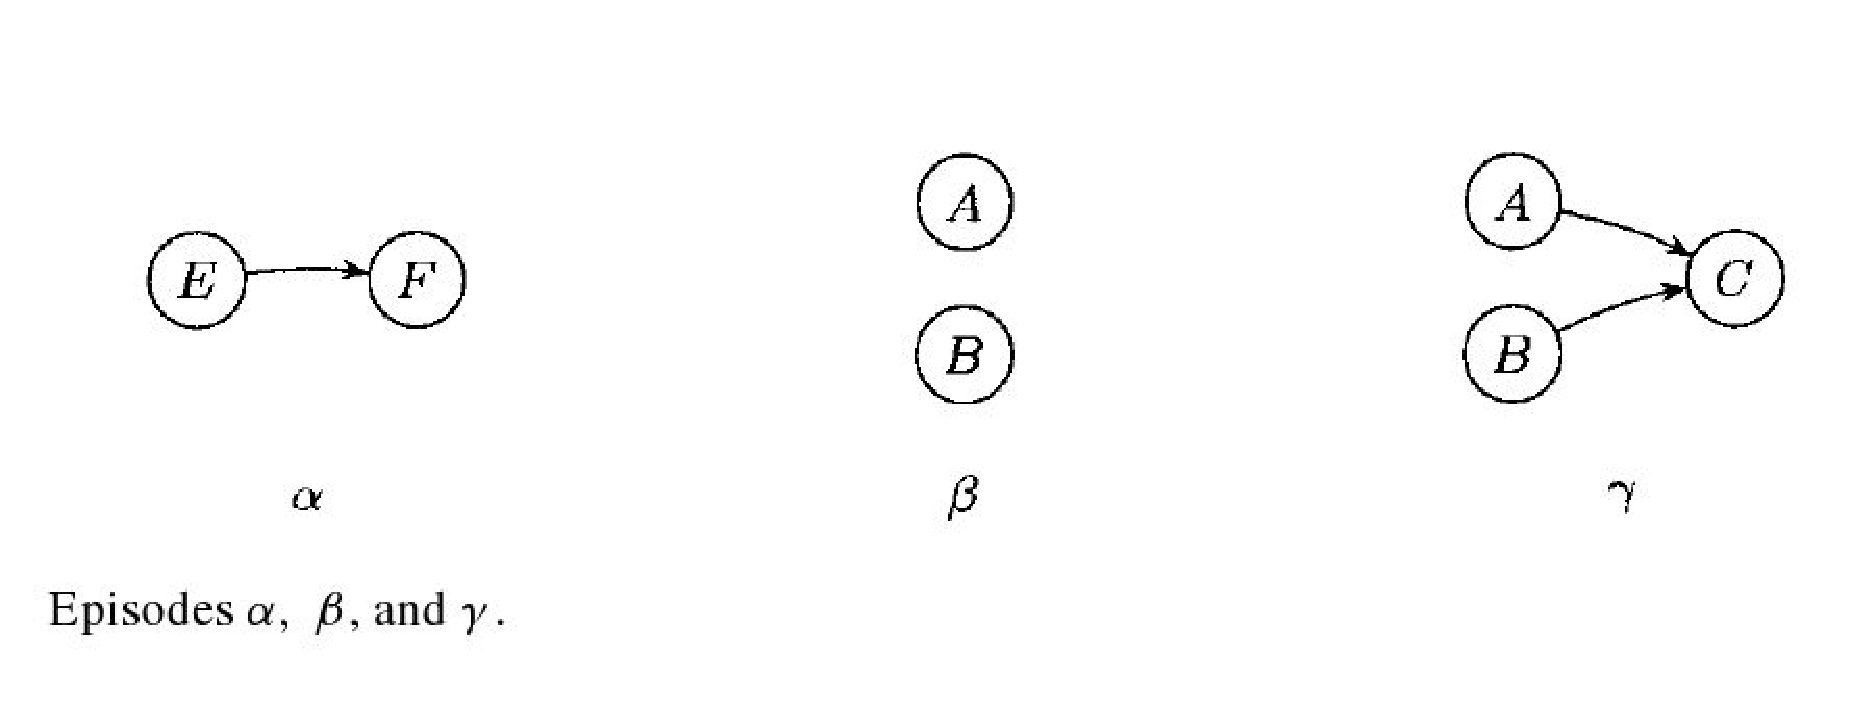
\includegraphics[scale=0.2]{patEpisodes.eps}
	\end{center}
    \item Для каждого эпизода считается частота: 
	    \begin{center}
	  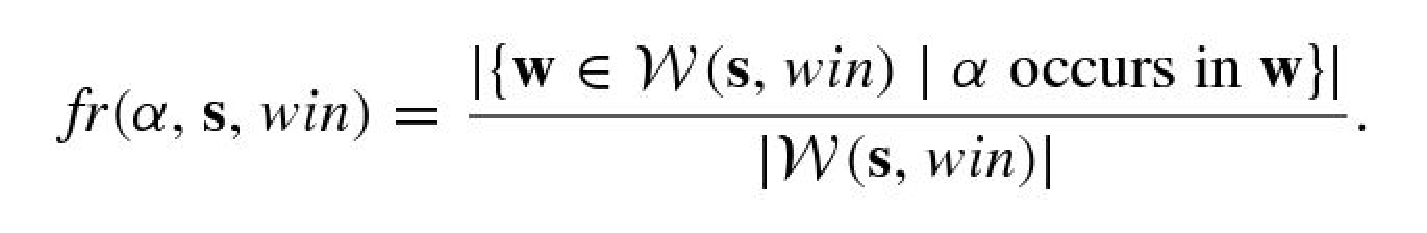
\includegraphics[scale=0.2]{episodesFormula.eps}
	  \end{center}
  \end{itemize}
\end{frame}

\begin{frame}
  \frametitle{Поиск}
  \begin{itemize}
    \item Выбираются простейшие события,
    \item для каждой пары событий проверяют их связанность. (Confidence)
  \end{itemize}
\end{frame}

\begin{frame}
  \frametitle{Особенности}
  \begin{itemize}
    \item Нету временных интервалов. Проход окном;
    \item Определяется только структура, последовательность связи в паттернах.
  \end{itemize}
\end{frame}

\subsection{Мотивы в нейронной активности}
\begin{frame}
  \frametitle{Эксперимент}
  <<Identifying repeating motifs in the activation of synchronized bursts
 in cultured neuronal networks>>.
 Nadav Raichman, Eshel Ben-Jacob. Journal of Neuroscience Methods 170
 (2008)96-110
  \begin{itemize}
    \item В чашку Петри ставят датчики, каждый из которых может регестрировать активность нескольких нейронов;
    \item спайки объединяются по времени в пачки;
    \item каждая пачка представляет распространение активности по нейронам;
    \item метрика на множестве пачек;
    \item пачки кластеризуются. Каждый кластер определяет паттерн.
  \end{itemize}
\end{frame}

\begin{frame}
  \frametitle{Визуализация}
  \begin{center}
	  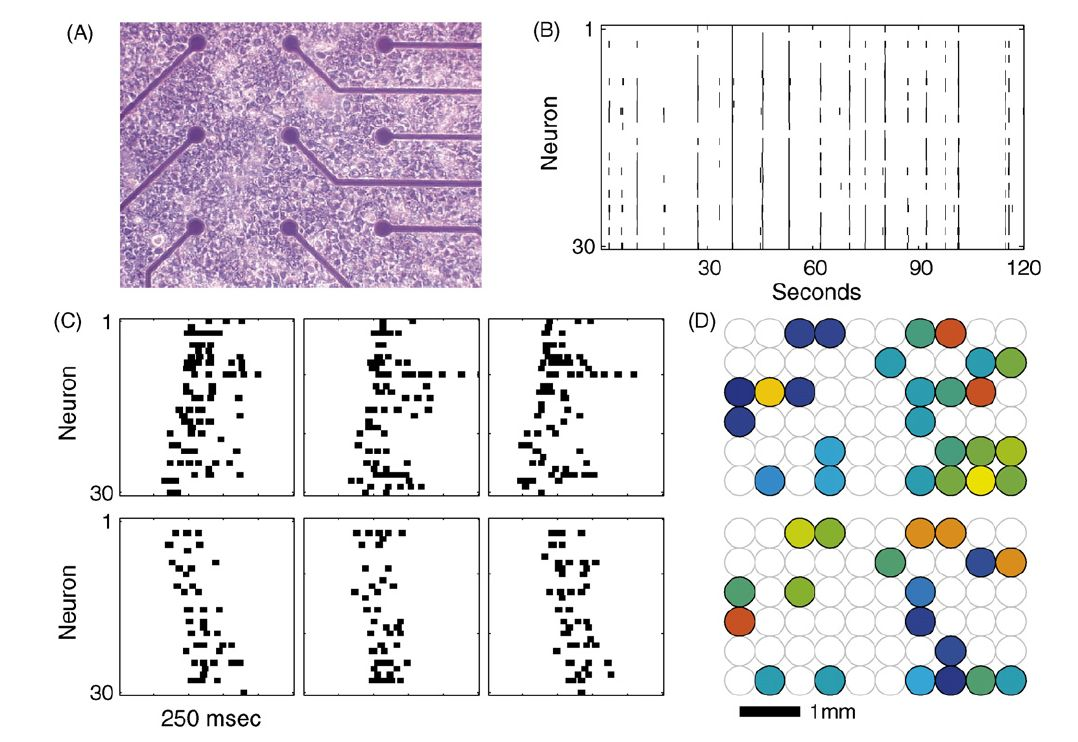
\includegraphics[scale=0.2]{motif.eps}
	\end{center}
\end{frame}

\begin{frame}
  \frametitle{Дендограмма}
  \begin{center}
	  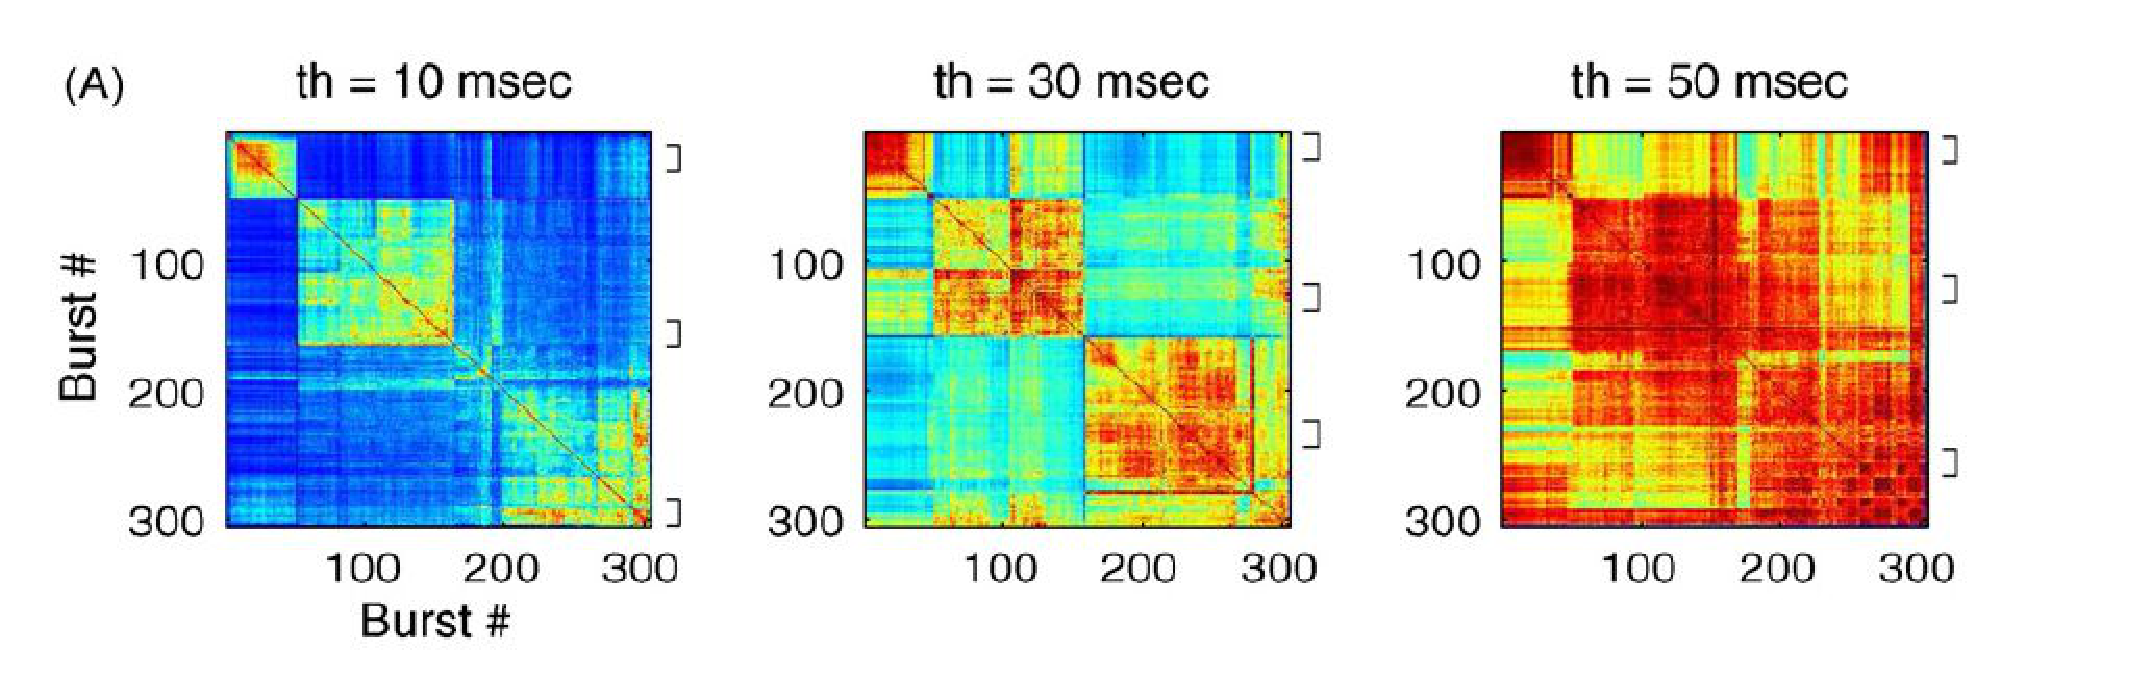
\includegraphics[scale=0.25]{motif_dend.eps}
	\end{center}
\end{frame}

\subsection{Геном}
\begin{frame}
\begin{itemize}
    \item Входные данные: последовательность аминокислот или нуклеотидов,
    \item дот-матрица $M=(m_{ij}),$ где $m_{ij}=0$, если $i$-й элемент первой последовательности не равен $j$-у 
    элементу второй последовательности, иначе $m_{ij}=1$. \\
    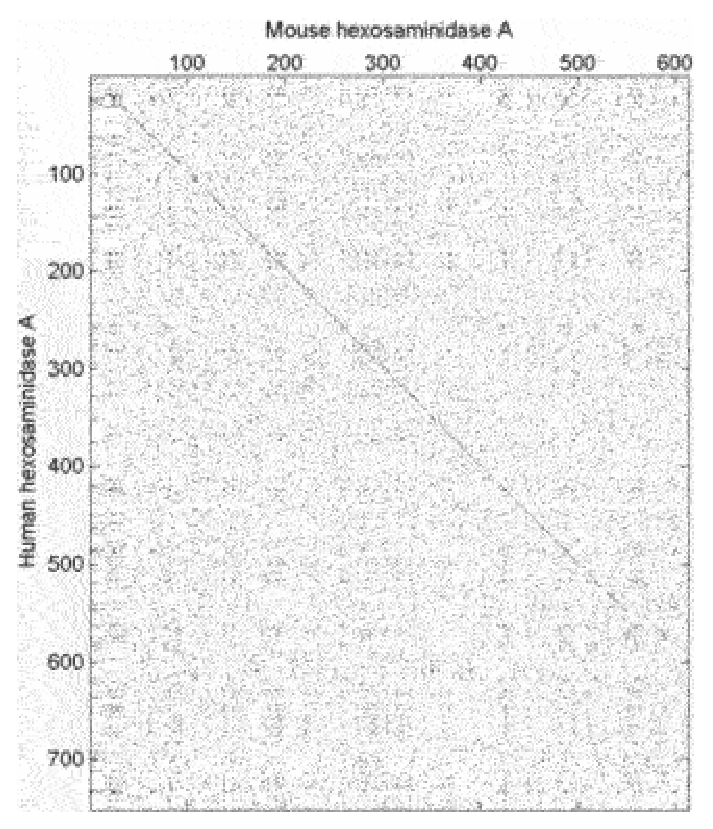
\includegraphics[scale=0.22]{plot.eps}
    \item Спектрально-аналитический метод.
\end{itemize}      
\end{frame}


\end{document}
